
\section{2D/ 3D, DdQq models}

As was mentioned before – the velocities in the LGCA are discrete. The same idea we have in LBM, the discretization of the velocities are all similar and described with DdQq model. For example we have such models as D2Q5, D2Q7, D2Q9, D2Q15, D3Q15, D3Q19 and D3Q27. If we have D2Qq then it means that we have two dimensions and D3Qq – 3 dimensions.

D2Q9 is the model with 9 directions (one center for particles at rest, four directions along the axes and four diagonal directions, see left illustration in Fig. 3), D3Q27 model has 27 directions (one center, six directions along the axes, 12 combinations of two axes and 8 combinations of three axes, see right illustration in Fig. 3).

\begin{figure}[H]
  \centering
  \begin{subfigure}[h]{0.3\textwidth}
    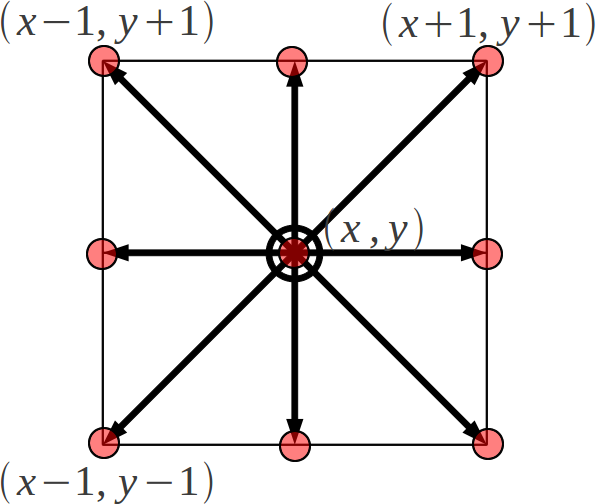
\includegraphics[width=\textwidth]{img/fig6-1.png}
  \end{subfigure}
  \begin{subfigure}[h]{0.3\textwidth}
    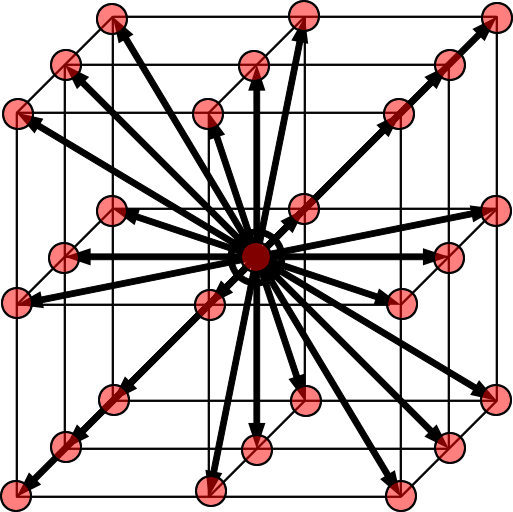
\includegraphics[width=\textwidth]{img/fig6-2.png}
  \end{subfigure}
  \caption{D2Q9 and D3Q27 velocity discretization models.}
\end{figure}

After the discretizing of the microscopic velocity space we get system of N-1 equations, which is easier to solve then Navier-Stokes equations. N is the amount of probability densities(distribution functions). This system of equations is a hyperbolic system of equations. On the figure 4 you can see the streaming step on D2Q9 model, which is described by the next functional:
\begin{equation}
f_i^{in}(\vec{r}+\vec{c}_{i}\Delta t, t+\Delta t) = f_i^{out}(\vec{r}, t)
\end{equation}

\begin{figure}[H]
  \centering
  \begin{subfigure}[h]{0.3\textwidth}
    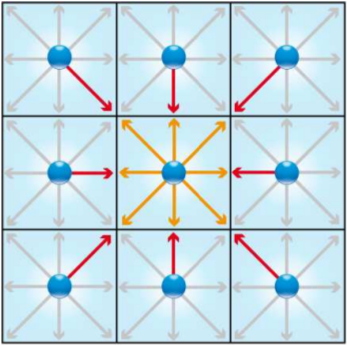
\includegraphics[width=\textwidth]{img/fig7-1.png}
  \end{subfigure}
  \begin{subfigure}[h]{0.3\textwidth}
    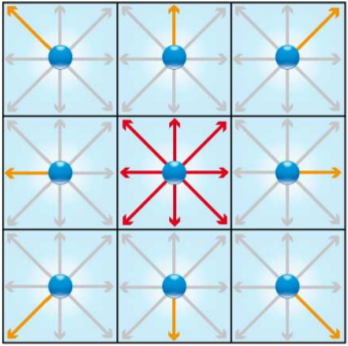
\includegraphics[width=\textwidth]{img/fig7-2.png}
  \end{subfigure}
  \caption{Streaming step [1].}
\end{figure}
